\subsubsection{Mechanical System}

\paragraph{Frame} \ \\
\vspace{-0.5cm}

Kamikaze’s frame (Figure \ref{fig:frame}) is designed using a cuboid aluminum V-extrusion structure, providing a stable and modular foundation for mounting various components. The 20×20 and 20×40 aluminum extrusions offer a strong yet lightweight framework that maintains structural integrity in underwater conditions.

\hspace{10pt} To enhance stability and buoyancy, HDPE side frame sheets (Figure \ref{fig:side_frame}) are integrated into the design. These sheets not only contribute to the aesthetic appeal of the ROV but also help in maintaining balance during operations. Their strategic placement ensures that the ROV remains hydrodynamically stable while supporting the overall structural framework.

\hspace{10pt} The frame is designed with precise mounting slots, allowing secure positioning of thrusters, cameras, and operational tools while maintaining easy access for maintenance. The bolted assembly ensures that components can be reconfigured or replaced without permanent modifications.

\hspace{10pt} Additionally, the frame is tailored for the E-JUST Robotics team, ensuring compatibility with the mission requirements of the MATE ROV competition while balancing durability, weight efficiency, and adaptability.

\begin{figure}[t]
    \centering
    \begin{subfigure}[b]{0.45\columnwidth}
        \includegraphics[width=\textwidth]{Sections/2Design Rationale/images/side frame.png}
        \caption{HDPE Side Frame.}
        \label{fig:side_frame}
    \end{subfigure}
    \hfill
    \begin{subfigure}[b]{0.5\columnwidth}
        \includegraphics[width=\textwidth]{Sections/2Design Rationale/images/frame.png}
        \caption{Aluminum Extrusion Frame.}
        \label{fig:frame}
    \end{subfigure}
    \caption{Kamikaze's Frame Illustration.}
    \label{fig:full_frame}
\end{figure}

\vspace{-0.3cm}
\paragraph{Propulsion} \ \\
\vspace{-0.5cm}

Kamikaze is equipped with seven T200 Blue Robotics thrusters, strategically placed to achieve six degrees of freedom for precise maneuverability (Figure \ref{fig:dof}). This setup balances performance, power consumption, and cost-efficiency, ensuring mission success without excessive energy use.

\hspace{10pt} Using seven thrusters instead of a larger number reduces power draw while maintaining stability and control. Each thruster's power consumption is affected by drag force, given by:

\begin{equation}
    F_d = \frac{1}{2} C_d \rho A v^2
    \label{eq:drag_force}
\end{equation}

Where:

\vspace{-0.5\baselineskip}
\begin{itemize}
    \setlength{\itemsep}{0pt}
    \item \(F_d\) = Drag force (N)
    \item \(C_d\) = Drag coefficient (ROV shape-dependent)
    \item \(\rho\) = Water density (kg/m\(^3\))
    \item \(A\) = Cross-sectional area (m\(^2\))
    \item \(v\) = ROV velocity (m/s)
\end{itemize}

\begin{figure}[h]
    \centering
    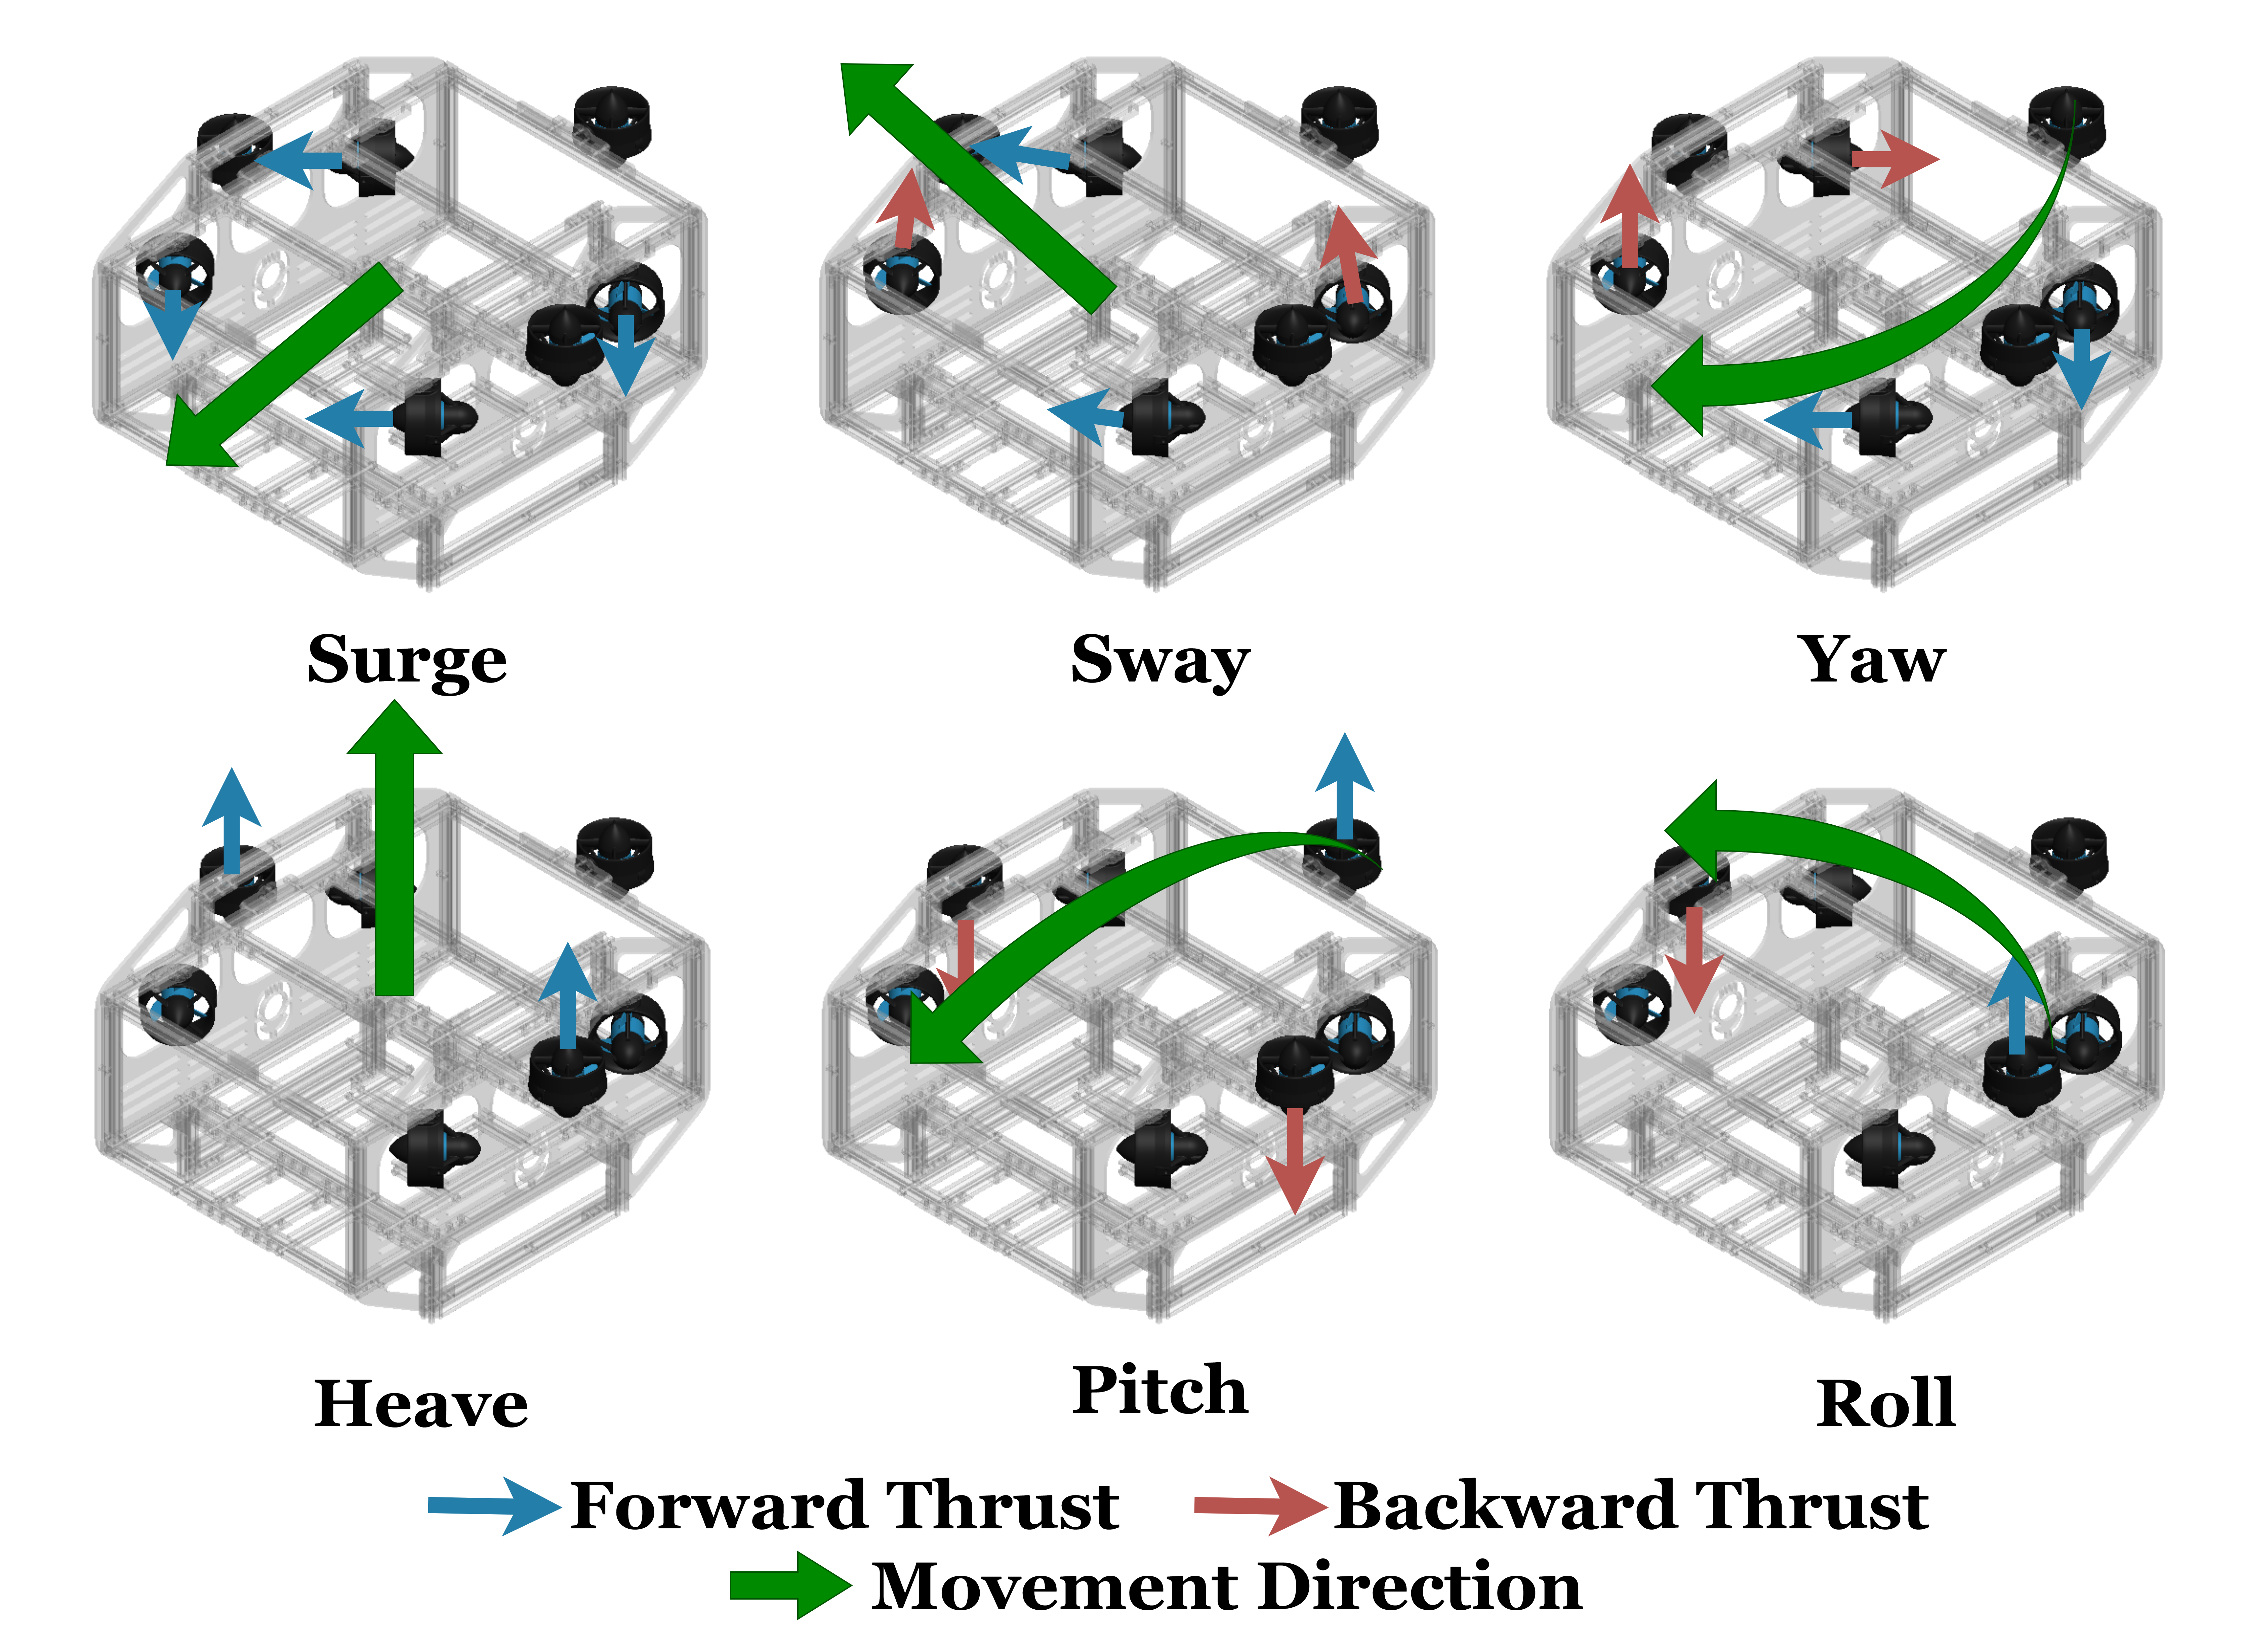
\includegraphics[width=\columnwidth]{Sections/2Design Rationale/images/dof.png}
    \caption{Kamikaze’s Degrees of Freedom.}
    \label{fig:dof}
\end{figure}

A CFD flow simulation was conducted to analyze water flow around Kamikaze (Figure \ref{fig:cfd}), minimizing drag and enhancing hydrodynamic efficiency.

\begin{figure}[b]
    \centering
    \rule{0.8\columnwidth}{4cm}
    \caption{Flow Simulation.}
    \label{fig:cfd}
\end{figure}

\vspace{0.2cm}
\textbf{Trade-offs in Thruster Selection}
\vspace{-0.5\baselineskip}
\begin{itemize}
    \setlength{\itemsep}{0pt}
    \item \textbf{Power vs. Performance:} More thrusters improve stability but increase power consumption. Seven thrusters provide a balance between efficiency and control.
    \item \textbf{Cost vs. Mission Needs:} Reusing last year’s T200 thrusters reduces costs while still meeting competition requirements.
\end{itemize}

\vspace{-0.3cm}
\paragraph{Buoyancy and Stability} \ \\
\vspace{-0.5cm}

Something about buoyancy and stability. \lipsum[1]

\begin{figure}[h]
    \centering
    \rule{0.8\columnwidth}{4cm}
    \caption{Buoyancy.}
    \label{fig:buoyancy}
\end{figure}

\vspace{-0.3cm}
\paragraph{Main Canister} \ \\
\vspace{-0.5cm}

The canister serves as the primary enclosure for the ROV, protecting essential components such as microcontrollers, power systems, and sensors while ensuring pressure resistance, corrosion protection, and ease of maintenance. The design consists of a 3D-printed PETG body, an aluminum base, and a PETG lid with embedded acrylic windows, providing structural stability and waterproof integrity under operational conditions.

\begin{figure}[h]
    \centering
    \includegraphics[width=0.6\columnwidth]{Sections/2Design Rationale/images/canister.png}
    \caption{Kamikaze’s Main canister.}
    \label{fig:canister}
\end{figure}

\hspace{10pt} PETG was chosen as a cost-effective alternative to aluminum, offering a balance between mechanical strength and manufacturability. Although PETG is inherently waterproof, Sikadur®-31 CF sealant was applied to enhance structural integrity and reliability. The 3mm-thick aluminum base provides structural support for bulkhead glands, preventing layer separation and ensuring durability. The canister dimensions are 276×276×142.59 mm, optimized for component housing and pressure resistance. A three-stage sealing process was implemented, consisting of mechanical fastening, epoxy bonding, and polyurethane sealant, to maintain a watertight enclosure. The removable PETG lid, secured with M5 screws and dual O-rings, allows for easy inspection and maintenance, while four embedded acrylic windows provide visual access without disassembly.

\hspace{10pt} To evaluate structural performance, a Finite Element Analysis (FEA) was conducted:

\vspace{-0.5\baselineskip}
\begin{itemize}
    \setlength{\itemsep}{0pt}
    \item \textbf{Top View (Figure \ref{fig:top_fda}):} Stress is concentrated around circular openings and edges, which experience higher mechanical loads from water pressure.
    \item \textbf{Bottom View (Figure \ref{fig:bottom_fda}):} Bolted connections and interface zones between the base and side walls accumulate stress, making them susceptible to deformation.
\end{itemize}

\begin{figure}[h]
    \centering
    \begin{subfigure}[b]{0.45\columnwidth}
        \rule{\textwidth}{4cm}
        \caption{Top View Analysis.}
        \label{fig:top_fda}
    \end{subfigure}
    \hfill
    \begin{subfigure}[b]{0.45\columnwidth}
        \rule{\textwidth}{4cm}
        \caption{Bottom View Analysis.}
        \label{fig:bottom_fda}
    \end{subfigure}
    \caption{Main Canister Finite Element Analysis.}
    \label{fig:fda}
\end{figure}

\vspace{-0.3cm}
\paragraph{Sealing Strategy} \ \\
\vspace{-0.5cm}

Something about sealing strategy. \lipsum[1]

\begin{figure}[h]
    \centering
    \rule{0.8\columnwidth}{4cm}
    \caption{Sealing.}
    \label{fig:sealing}
\end{figure}

\vspace{-0.3cm}
\paragraph{Cameras} \ \\
\vspace{-0.5cm}

Something about cameras. \lipsum[1]

\begin{figure}[h]
    \centering
    \rule{0.8\columnwidth}{4cm}
    \caption{Cameras.}
    \label{fig:cameras}
\end{figure}

\vspace{-0.3cm}
\paragraph{Grippers} \ \\
\vspace{-0.5cm}

Something about grippers. \lipsum[1]

\begin{figure}[h]
    \centering
    \rule{0.8\columnwidth}{4cm}
    \caption{Grippers.}
    \label{fig:grippers}
\end{figure}